\chapter{Measurement Techniques}
We have characterized the performance of \gls*{ps} frequency stabilisation using a number of methods which are detailed here. Spectral linewidth is the principle metric by which stabilisation techniques are compared...

{\color{red}More detail in this intro.}

\section{Heterodyne Methods}

Heterodyning is a technique, invented by Canadian Reginald Feessenden in 1901, which mixes two frequencies to produce a new frequency. {\color{red} [get proper citation, this is from Wiki]} In optics the technique can be used to examine the spectral properties of two lasers.~{\color{red}[Citation?]}

\subsection{Basic Theory}
In the electrical signals context heterodyning involves the `mixing' or multiplying of two signals (e.g. two sine waves) to produce two different signals with frequencies equal to the difference and sum of the original frequencies:
\begin{equation}
\sin(\theta_1)\sin(\theta_2) = \frac{1}{2} \cos(\theta_1-\theta_2) - \frac{1}{2} \cos(\theta_1+\theta_2).
\end{equation}

In the optical context this is achieved due to the interference term accrued when squaring the electric field in order to calculate the intensity detected by the photodetector. The intensity of an electric field is given by:
\begin{equation}
I(t) = \frac{c\epsilon_0}{2}|E|^2.
\end{equation}

For two copropagating lasers with electric fields $E_{1, 2}$ and angular frequencies $\omega_{1, 2}$ we can write
\begin{equation}
E_{i}(t) = \sin(2\pi \omega_{i}).
\end{equation}
The electric field at the detector, $E_T$, is given by the sum of $E_{1}$ and $E_{2}$, and thus the intensity is given by,
\begin{align}
I(t) &= |E_1(t) + E_2(t)|^2\nonumber\\
&= E_1(t)^2 + E_1(t)E_2(t) + E_2(t)^2.
\end{align}
The interference term, $E_1(t)E_2(t)$, allows heterodyning of optical signals.

\subsection{Optical Heterodyne Methods}

There are a number of linewidth measurement techniques that utilise heterodyning. The major ones are:
\begin{itemize}
\item Heterodyne beatnote with two identical lasers.
\item Heterodyne beatnote between laser of interest and a relatively narrow reference laser.
\item Self-heterodyne beatnote of a laser with itself.
\end{itemize}

\subsection{Linewidth Discrepancies}
{\color{red}I'm not certain enough about what's going on here so just remove this.}

There is an interesting discrepancy between intuition and what the literature uses to describe `linewidth'.
Intuitively, when discussing the spectral properties of light, one would expect references to refer to the properties of the electric field since that is the entity that is interacting with atoms and other frequency references.
However, the literature seems to exclusively refer to properties of the power of the signal from photodetectors, as shown on spectrum analysers, which differ by a factor of 2 which will be shown below.
Despite this fact this document follows the convention to avoid confusion.

The simplest way to examine a heterodyne signal is to look at the signal from the detector on a radio-frequency spectrum analyser.
A spectrum analyser shows the power for each frequency component of the input electrical signal.
The power of the electrical signal from the detector, $P_{elec}$ is roughly:
\begin{equation}
P_{elec}\propto I^2 \propto E^2
\label{eq:beatnote_proportional}
\end{equation}
where $I$ is the light intensity incident on the detector and $E$ is the electric field incident on the detector.

Of primary interest are the spectral properties of these signals which are given by their Fourier transform.
However we cannot simply write
\begin{equation}
\mathcal{F}[P_{elec}]\propto \mathcal{F}[I^2] \propto \mathcal{F}[E^2]
\end{equation}
since it's not true.
The inverse convolution theorem, however, can be used
\begin{equation}
f\cdot g = \mathcal{F}^{-1} \bigg[ \mathcal{F}[f] \otimes\mathcal{F}[g]\bigg].
\end{equation}

So Eq. \ref{eq:beatnote_proportional} in Fourier space becomes
\begin{align}
\mathcal{F}[P_{elec}]&\propto \mathcal{F}[I]\otimes\mathcal{F}[I]\nonumber\\
&\propto \big\{\mathcal{F}[E] \otimes\mathcal{F}[E]\big\} \otimes\big\{\mathcal{F}[E] \otimes\mathcal{F}[E]\big\}
\end{align}

For a Gaussian lineshape beatnote with \gls{rms} width $\sigma$, we can write
\begin{equation}
\mathcal{F}[E] = A e^{-(f-f_0)^2/2\sigma^2}.
\end{equation}

It is easy to show that the convolution of two Gaussians produces another Gaussian with variance equal to the sum of the variance of the two constituent functions.
Thus,
\begin{equation}
\mathcal{F}[I] = B e^{-(f-f_0)^2/4\sigma^2}
\end{equation}
and
\begin{align}
\mathcal{F}[P] &= B e^{-(f-f_0)^2/8\sigma^2}\nonumber\\
&= B e^{-(f-f_0)^2/2(2\sigma)^2}
\end{align}
So the width of the signal shown on a spectrum analyser has twice the spectral width of the electric field that generated it.

\begin{figure}
\centering
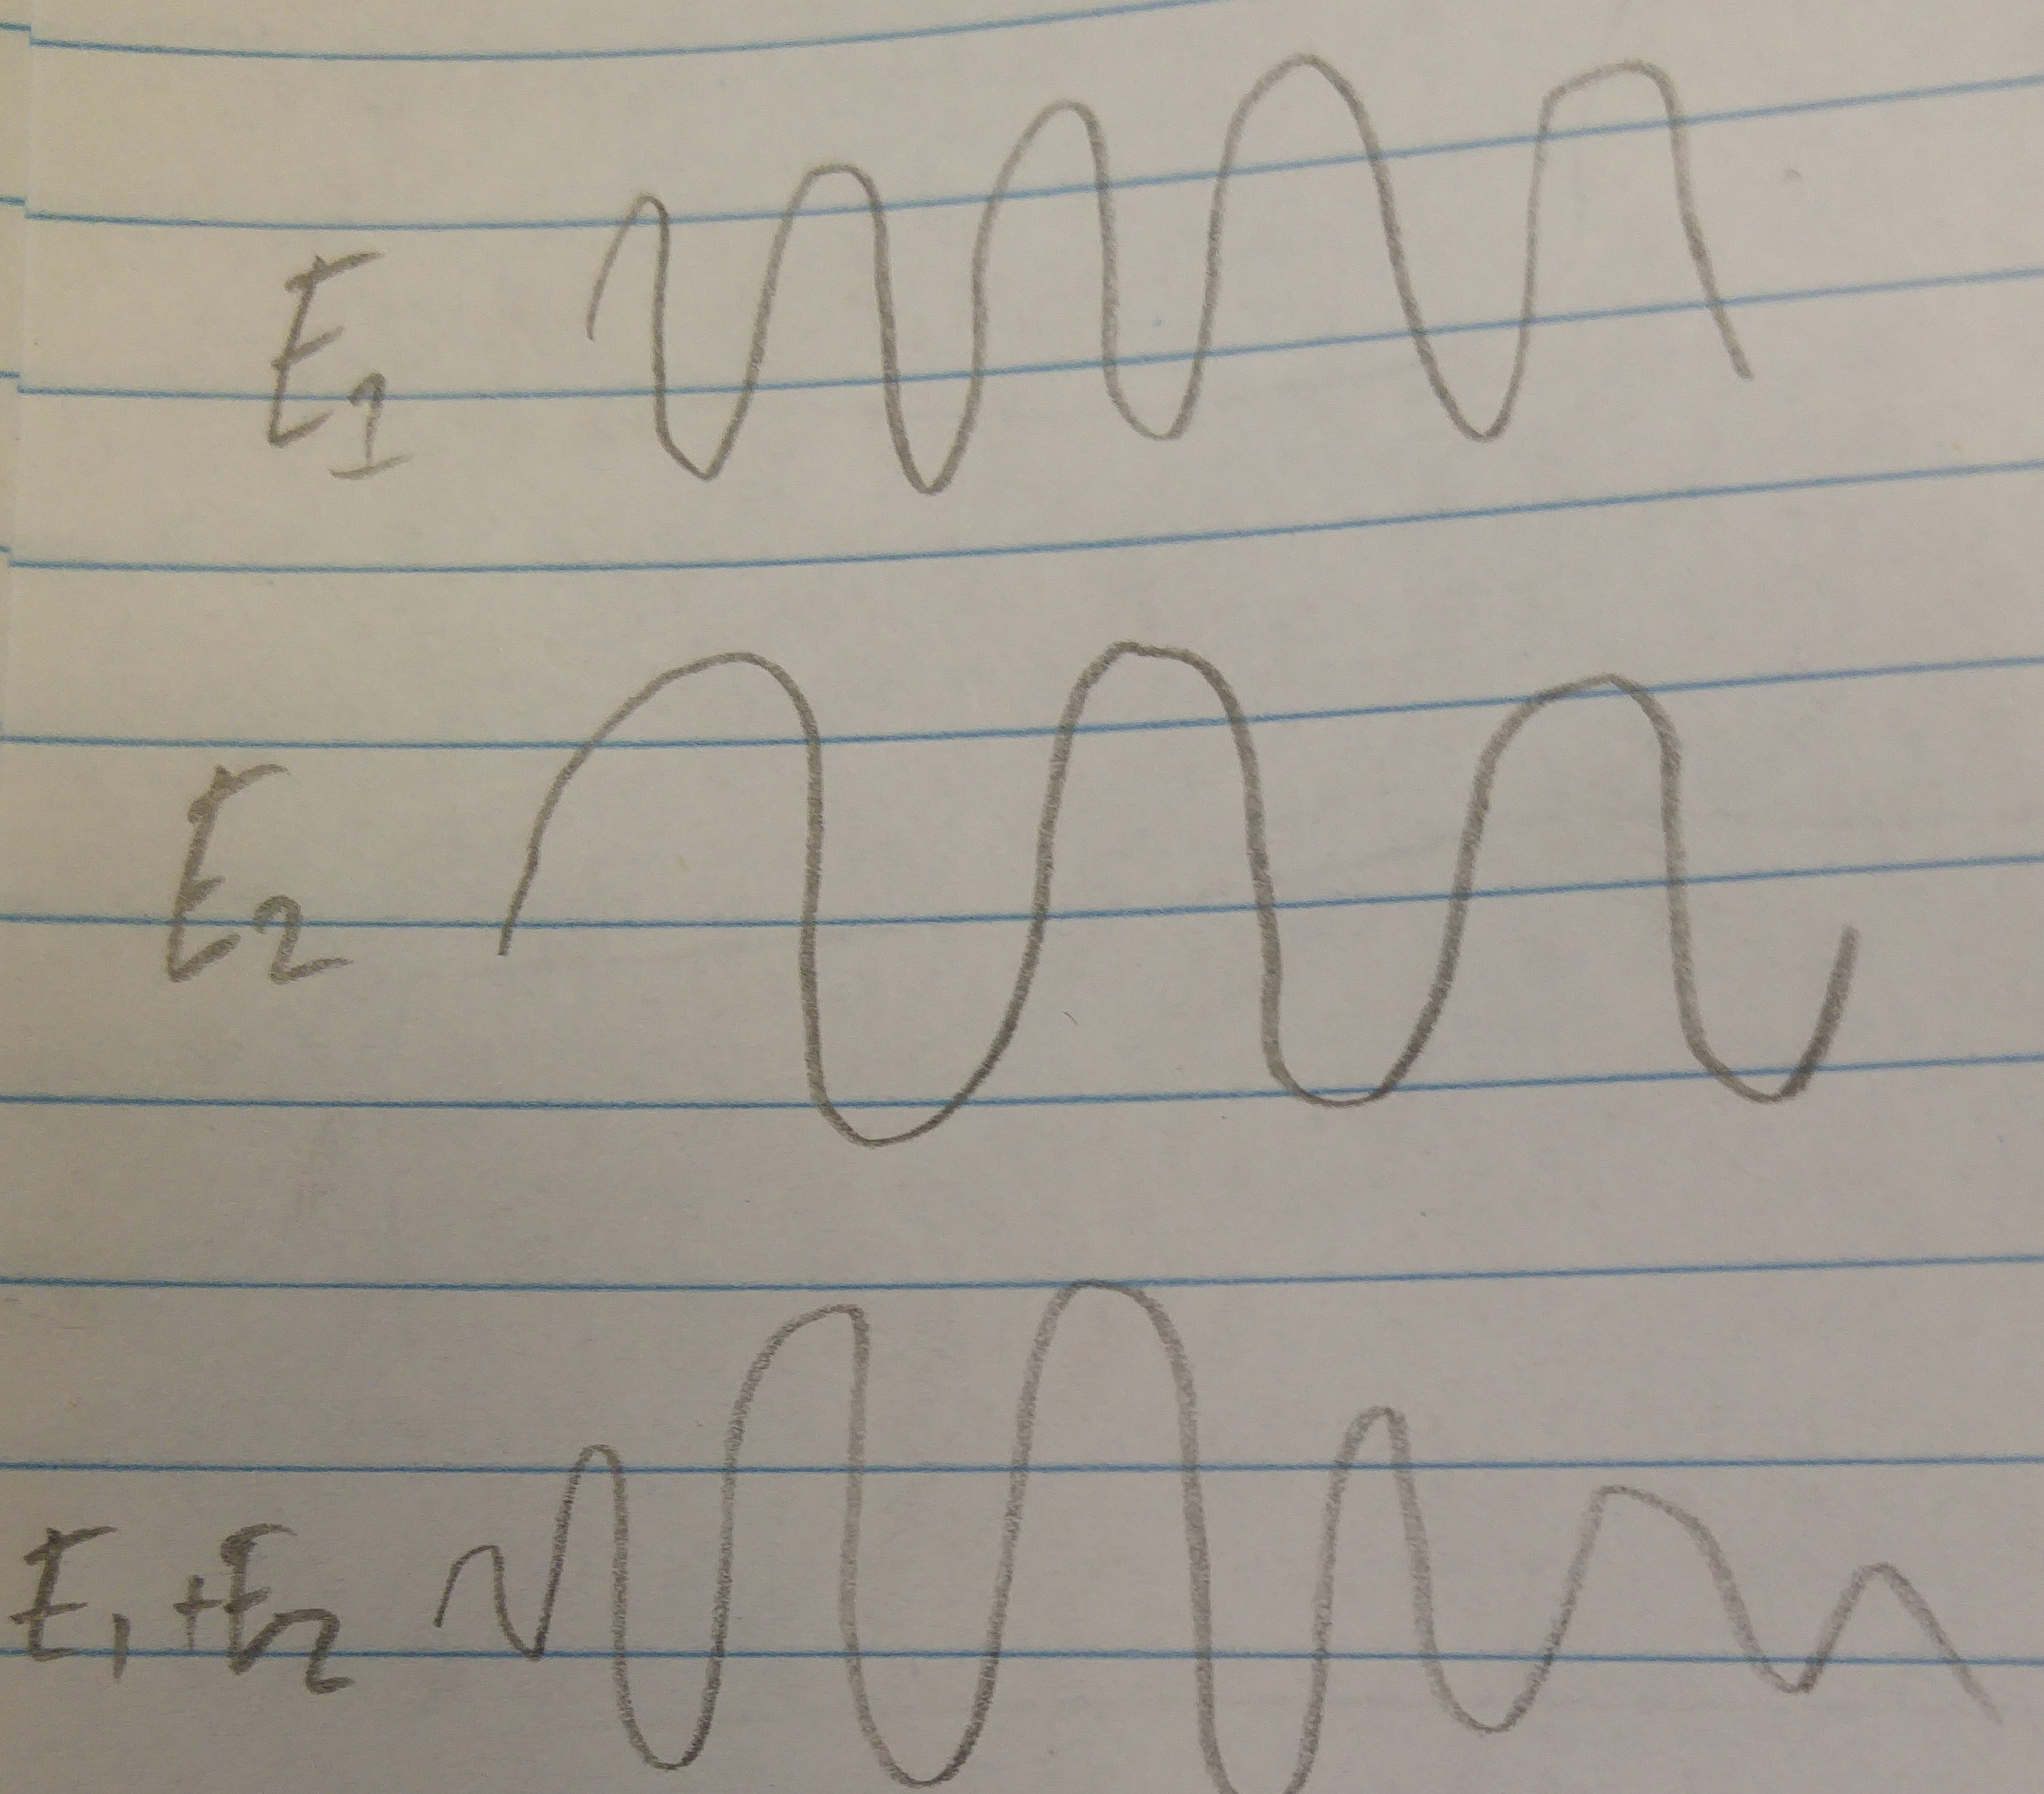
\includegraphics[width=0.5\linewidth]{part1/Figs/beatnote.jpg}
\caption{Depiction of simple beatnote.}
\label{figure:simple_beatnote}
\end{figure}

\subsection{Self-heterodyne}

Self-heterodyne is...

Single delay...

How much delay?

Multipass delay...

These are the results I got...

They look good... too good.

Here's why...\cite{richter_linewidth_1986}

\section{Frequency Reference}
\begin{itemize}
\item Identical laser
\item Narrow laser
\item Three Gaussian lasers
\end{itemize}

\section{Noise measurements}

\section{Bandwidth Stuff}

\section{Long Term Stability}

\subsection{Fibre Stability}

Make some measurements of how the fibres behave over time. Map it to the frequency stability of PS.

